
% Research and Analyse!
% Show Specialist Knowledge!
% Communicate Effectively!
% Experiment Effectively!

% TODO: research at http://vulkan.gpuinfo.org/
% TODO: gantt chart: https://www.excel-easy.com/examples/gantt-chart.html
% TODO: Identify the best of my academic writing style here and replicate it in the rest of the paper.
% TODO: Code colors: https://www.overleaf.com/learn/latex/Code_Highlighting_with_minted

\documentclass[11pt, a4paper, twocolumn]{article}
\usepackage[T1]{fontenc}
\usepackage[utf8]{inputenc}
\usepackage{titlesec}
\usepackage{natbib}
\usepackage{graphicx}
\usepackage{hyperref}
\usepackage{graphicx}
\usepackage[font={small, it}, labelfont=bf, center]{caption}
\usepackage[top=1cm, left=1cm, right=1cm, bottom=2cm]{geometry}

\usepackage{helvet} % Helvetica 'phv'
\usepackage{mathptmx} % Times 'ptm'

\urlstyle{same}

\titleformat{\section}
  {\sffamily\bfseries\Large} % format
  {\thesection} % label
  {1em} % label separation
  {} % before-code

\titleformat{\subsection}
  {\sffamily\bfseries} % format
  {\thesubsection} % label
  {1em} % label separation
  {} % before-code

\title{\sffamily\bfseries An Exploration of Optimisation Techniques\\for Vulkan-based Particle Systems}
\author{Robin Wragg}
\date{\today}

\begin{document}

\maketitle
%%%%%%%%%%%%%%%%%%%%%%%%%%%%%%%%%%%%%%%%%%%%%%%%%%%%%%%%%%%%%%%%%%%%%%%%%%%%%%%%

\section{Introduction}

The aim of this project is to research and experiment with techniques for optimising the rendering speed of particle systems and Vulkan-based rendering pipelines. Techniques are collected from related literature and are applied to our own program, a particle system built in C++ and Vulkan. From this experience, and independent experimentation, we will collect and document the most appropriate techniques for easy consumption by those who may be considering implementing or improving their own particle system and/or Vulkan pipeline.

Multiprocessors will briefly be explored in the literature review, but this paper will be focussing on consumer-oriented systems with a single, multi-core CPU and a single GPU throughout this paper.

\subsection{Particle Systems}

Various ephemeral phenomena such as fire, rain, explosions and smoke can be challenging to render convincingly and efficiently using the mesh-of-triangles approach that is used for solid objects.

Creating an accurate simulation of these phenomena is impossible to do in real-time, because it would require representing many trillions of individual molecules; completely prohibitive from a performance perspective. Particle systems are a way of approximating the behaviour of these systems. The technique involves rendering many \emph{particles} (discrete, simple objects) per frame; the number of particles is dependant on the intended realism/quality and the required rendering speed. Particle systems are more versatile than just a way to simulate realistic visual effects; they are often used to render unrealistic phenomena, such as magical effects.

A particle can be any simple, renderable object; \emph{billboards} (flat, textured polygons that always face the camera) are perhaps the most common kind of particle, and can represent an individual droplet of rain or a section of a cloud. But a particle can be anything the framerate allows; even traditional meshes can be used, if the amount and complexity are low enough for real-time rendering.

Particle systems are a useful environment for experimenting with performance because the faster the particles render, the more particles are able to be rendered without a noticeable drop in framerate, allowing improved visual results. This quantitative nature makes them appropriate for quantifying the performance impact of any changes made to the program.
% "allowing improved visual results" Why? Does more mean better?

\subsection{Real-time Graphics Pipelines}

(todo)

\subsection{The Vulkan API}

Vulkan is a cross-platform Application Programming Interface for rendering 3D graphics in real-time \citep{Vulkan}. It is developed by the non-profit consortium, the Khronos Group \citep{Khronos}. Along with its contemporaries, Microsoft DirectX 12 \citep{dX12} and Apple Metal \citep{AppleMetal}, it exists to provide graphics programmers with more control over the entire graphics pipeline, enabling a better balance in workload between the CPU and GPU. This was in response to its precursors, namely DirectX 11 \citep{dx11} and OpenGL \citep{OpenGL}, which were often bottlenecked by the single-threaded performance of the CPU \citep{CpuBottleneck}.

% TODO: Mention SPIR-V etc?

\subsection{Multi-threading}

% TODO: illustrate Amdahl's law
\begin{figure}[h]
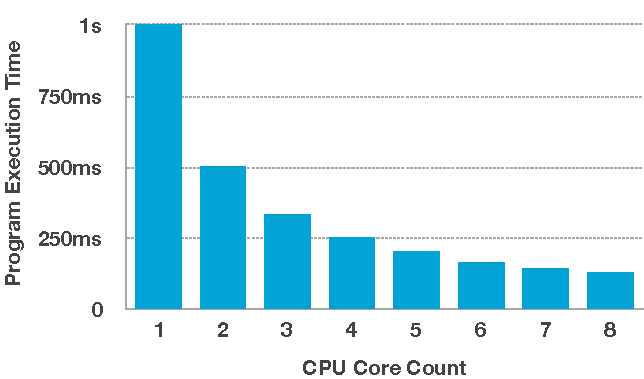
\includegraphics[width=\linewidth]{cpu_cores}
\caption{Theoretical best-case execution time of a program that requires one second of CPU time, by CPU core count.}
\label{fig:cpu_cores}
\end{figure}

Concurrent execution is the very common technique in modern computing of running multiple threads in a single program; the effect is equivalent to two or more processes with access to the same memory. This allows a CPU with multiple cores to run more than one of these threads at once.

All modern consumer CPUs have at least two physical cores, so the performance of a program is can sometimes be over twice as slow as its potential if it doesn't utilise multiple threads effectively in its performance-critical sections. Or inversely, a single-threaded program that requires one second of CPU time can reach a fraction of that time if rewritten as a multi-threaded program, but every additional core yields diminishing returns (see Figure \ref{fig:cpu_cores}). % TODO: Explain why, and explain and cite Amdahl's law

\section{Literature Review}

% TODO: \subsection{Performance Profiling}?

\subsection{Particle System Design}
% TODO: show an image of Tatarchuk's work
\citet{Tatarchuk2006} has shown many impressive techniques for rendering various effects for a realistic rainy night in a city. Of particular note was skillful use of particles based on pre-blurred normalmaps to create transparent water droplets that have realistic specular highlights from the surrounding streetlights. This is used convincingly both as rain directly from the sky and also as more of a waterfall-like effect to show water gushing out of drainpipes. The water would then splash into puddles using a pre-rendered splash sequence. The otherwise easy-to-spot repetitiveness of this splash was hidden by randomising the size and transparency of those particles, as well as flipping them horizontally. This could perhaps be improved even further by making larger splashes animate slightly slower, so that the actual simulated falling speed of the droplets within the splash would be convincingly similar regardless of particle size. An additional visual improvement could involve spawning new, tiny droplets in a generally upward velocity at the point of the biggest splashes; this could emphasise the impact of the splash. % TODO: Delve into this paper more?

\citet{Boulianne2007} implemented a biological system simulator using a 3D grid in which each element can hold one or zero particles. Their simulator needed to take into account the spacial locality of particles; a grid facilitates this by removing the need for distance calculation and particle search. Although their implementation did not have real-time graphics in mind, this grid-based approach could be applied to particle-based rendering for situations where the intended effect requires particles to react to each other based on their proximity. (TODO: That's called spatial hashing!) Additionally, \citet{Boulianne2007} states ``this system is expected to be suitable for acceleration with parallel customizable hardware,'' meaning this technique would likely be appropriate for rendering real-time particle systems and the parallel nature of GPUs.

\subsection{Techniques for Efficient Real-time Graphics}

\citet{Crawford2018} noted that shader compiler optimisation can make a modest improvement to graphics performance, but it is highly dependent on shader code itself. With their test suite of the LunarGlass/LLVM optimisation framework and the GLSL shaders from GFXBench 4.0, they found that shaders can be sped up by as much as 25\% by finding the best combination of compiler flags, but 1-4\% should be expected in general. Common optimisations that shader compilers can perform are dead code elimination, factoring out conditionals, unrolling loops, coalescing multiple vector element assignments into a single swizzled (TODO: explain swizzling. VkImageViewCreateInfo uses it) vector assignment, global value numbering causing variable elimination, and simplifying arithmetic by reordering the statements. The study reviewed only source-to-source optimisations; source-to-machine-code optimisations weren't explored. Further speed-ups could be found in that area.

Referring to Vulkan and DirectX 12, \citet{Joseph2016} states ``the central focus of this new generation of APIs is to increase the amount of draw calls possible while decreasing the amount of overhead for the CPU.'' As graphics programmers, we can reinterpret this to indicate that it is critical to reduce the amount of time that the CPU and GPU are required to block each other to communicate, in order to get the most out of the hardware.

\subsection{Multi-threaded Software Design}

Coordination between threads is a necessary characteristic of reliable multi-threaded systems \citep{Powell}. Without coordination, race conditions and simultaneous unsafe memory accesses can occur, leading to unintended, unpredictable behaviour, often resulting in crashes due to memory access violations. Some ways to avoid these issues are presented below.

\textbf{Mutexes} are perhaps the most common mechanism to ensure thread coordination. A thread can attempt to \emph{lock} a mutex; if the mutex was previously in an unlocked state, the attempt to lock is successful and that thread can continue as normal. The thread now "owns" the mutex. If the mutex is already locked, in most cases the thread will be blocked, and will wait until another thread \emph{unlocks} the mutex (only the owning thread can unlock a mutex). The exception to this is when a \verb|try_lock()| function or equivalent is called on the mutex instead of \verb|lock()|; this will not block the thread, and will instead give the opportunity for the thread to do other work while it waits for  Not all mutex implementation have \verb|try_lock()|, but this functionality is available for this project as part of C++'s \verb|std::mutex| \citep{CppMutex}.

% Paragraph code example
% \begin{verbatim}
% int main() {
%   float a = 3.45;
%   char *str = "oaiwjef";
%   return 0;
% }
% \end{verbatim}

% TODO: talk about how I'm using semaphores in Vulkan
\textbf{Semaphores} come in various kinds, but in general they are thread-safe counters. Specifics as to how a semaphore is used is up to its API and the programmer's needs, but a common convention is for a thread to perform a \verb|wait()| operation on a semaphore, which will cause the thread to block until the semaphore's counter is greater than zero. At that point, or if it was already greater than zero, the semaphore will decrement by one and the thread will continue executing. A \verb|post()| can be performed by any thread, which will increment the semaphore. If the counter is above zero and there is at least one thread waiting on the semaphore, one thread can now continue as stated above \citep{BoostSync}.

A semaphore that is always either one or zero is equivalent to a mutex, except for one difference: A \verb|post()| operation can be performed by any thread that has access to the semaphore, allowing any thread to unblock execution, instead of just the thread which called \verb|wait()|.

Semaphores are being introduced into the C++ standard library as part of C++20 \citep{C20Sync}, so they aren't available to our C++17 environment but we could use a separate library for this functionality if necessary, such as the Boost library collection's \verb|interprocess_semaphore|, \verb|named_semaphore|, and \verb|anonymous_semaphore|.

% TODO: Talk in more detail about different kinds of thread blocking like deadlocking.
Blocked threads are a significant cause of the reduction of maximum theoretical performance on multi-core systems \citep{Alemany1992}. In the worst case, a \emph{deadlock} can occur when all threads are blocked, waiting on each other indefinitely. In the case of mutexes, a good rule of thumb is to keep the areas of the program that are mutex-guarded as small, simple and fast as possible, to reduce the amount of time that mutexes are locked, thereby reducing the chance of blocked threads.

Although the effects of thread-blocking can be a significant challenge to remove entirely, there exist programming techniques that allow concurrent sections to communicate without blocking each other, such as \emph{exponential backoff}, an algorithm commonly used in network coordination, that slows a process or thread in order to reduce congestion on a shared resource such as an Ethernet node \citep{Goodman2019}, or more applicably for us, a mutex or critical memory. This of course has the downside of one or more threads not operating at their maximum speed but it can have an overall benefit, depending on the bottlenecks of the program.

\emph{Optimistic concurrency control} is another class of algorithms for non-blocking concurrency that involves validating a transaction performed on shared data before committing it \citep{Herlihy1993} in an attempt to detect whether data corruption had occurred due to simultaneous writes or reads. Again, this has a downside of requiring extra work per transaction.

% "" (some of these techniques) are very complex; their usefulness must be weighed against the development team's ability to handle the additional complexity, and the cost of time spent implementing it. For this reason, we began implementing the optimisation techniques that appeared to have a good benefit-to-complexity ratio. % TODO: make a chart of these ratios?

% good structure from "SunOS Multithread Architecture": The remainder of this paper is divided into N sections. The first section gives an overview of the architecture and introduces our terminology. The second section discusses our design goals and principles. The third section gives additional details of operation and interfaces and how the UNIX process model is reinterpreted in the new environment. The fourth section gives some performance data and operational experience. The last section compares this architecture with others.

\section{Methodology}

% After examining the literature, we decided on a [something] implementation based on the techniques of cite, cite, cite, and cite.

\subsection{Equipment}

% TODO: rephrase this like a built a PC specifically for this project?
We will be designing, profiling and optimising the program for a desktop computer with an Intel Core i5 6400 at 2.7-3.3 GHz with four cores, 8GB of DDR4 RAM at (TODO: what frequency?) and an Nvidia Geforce GTX 1060 3GB. This  graphics card is the most common among Steam users with a 14.5\% share at the time of writing \citep{SteamSurvey}. Valve/Steam's published data on their users' CPUs suggests that at least 25\% of users own a CPU with the same core count and a similar frequency as our i5 6400. 8GB is also the most popular memory amount at 37.1\% of users, so this setup in all should give us a good example of how this program would perform on an average user's system.

% TODO: Note about the CPU not having more threads than cores? (4:4)

% TODO: Talk about how we will profile it. Vulkan layers, Visual Studio's tools etc.

\subsection{Performance Profiling}

% (Discuss how I'll be using Vulkan's validation layers, Visual Studio's profiling tools, and concurrency visualisation tools such as RAD Game Tools' Telemetry. Talk about what I'll be looking for when using each tool, and their strengths and weaknesses.)

\section{The Initial Implementation}

% (Describe the design decisions of the program before any optimisation is performed, and any Vulkan-specific implementation details relevant to the project.)
% My implementation never requires reallocating particles! Brag!

\section{Optimisation \& Analysis}

% (Describe in detail all the optimisation techniques I implemented and the changes in the performance characteristics of the program as I make changes to the code. Describe the critical thought processes along the way. Describe the complexity and other difficulties of implementing each optimisation. Towards the end of this section, focus on analysis including comparisons of related optimisations performed. Include charts showing how performance scales with the amount of particles. Include diagrams showing data pipelines.)

\section{Conclusion}

% (Continue to analyse as in the previous section but take a bigger-picture approach and summarise the overall findings. Write in a specific style knowing that some readers will have read the abstract and then jumped to this section.)


%%%%%%%%%%%%%%%%%%%%%%%%%%%%%%%%%%%%%%%%%%%%%%%%%%%%%%%%%%%%%%%%%%%%%%%%%%%%%%%%
\bibliographystyle{agsm}
\bibliography{mendeley_refs, other_refs}

% TODO: appendix entry with full details of the computer - include the protocol and theoretical speed of the GPU's bus etc.
% TODO: appendix entry with notes on Vulkan on macOS with MoltenVK

\end{document}





